% !TeX encoding = UTF-8
\chapter[Client]{Client}
\thispagestyle{fancy}
\label{client}

Die Beschreibung des Client bezieht sich im Folgenden nur auf die Applikation, welche Sprecher oder Zuhörer für die Präsentation zur Steuerung und Ansicht auf ihrem Endgerät benutzen. Client meint in diesem Zusammenhang nicht den vom Server gesteuerten Projektor.

\section[Grafische Benutzeroberfläche (GUI)]{Grafische Benutzeroberfläche (GUI)\footnote{Sascha Brexeler}}
\label{GUI}
Die Gestaltung dieser GUI bezweckt eine leicht verständliche, intuitiv bedienbare Oberfläche mit zielführender Benutzerführung und Hilfestellungen.
Die GUI ist für Geräte mit Android als Betriebssystem entwickelt, aber theoretisch nach dem kompilieren mit eventuell erforderlichen kleinen Anpassungen auch auf anderen Plattformen/Geräten ähnlich abgebildet und verwendbar. Erfolgreich getestet ist die App allerdings derzeit nur für Android (4.3 + 4.4) und Windows.


\begin{figure}[ht!]
	\centering
	\begin{minipage}{0.31\linewidth}
		\centering
		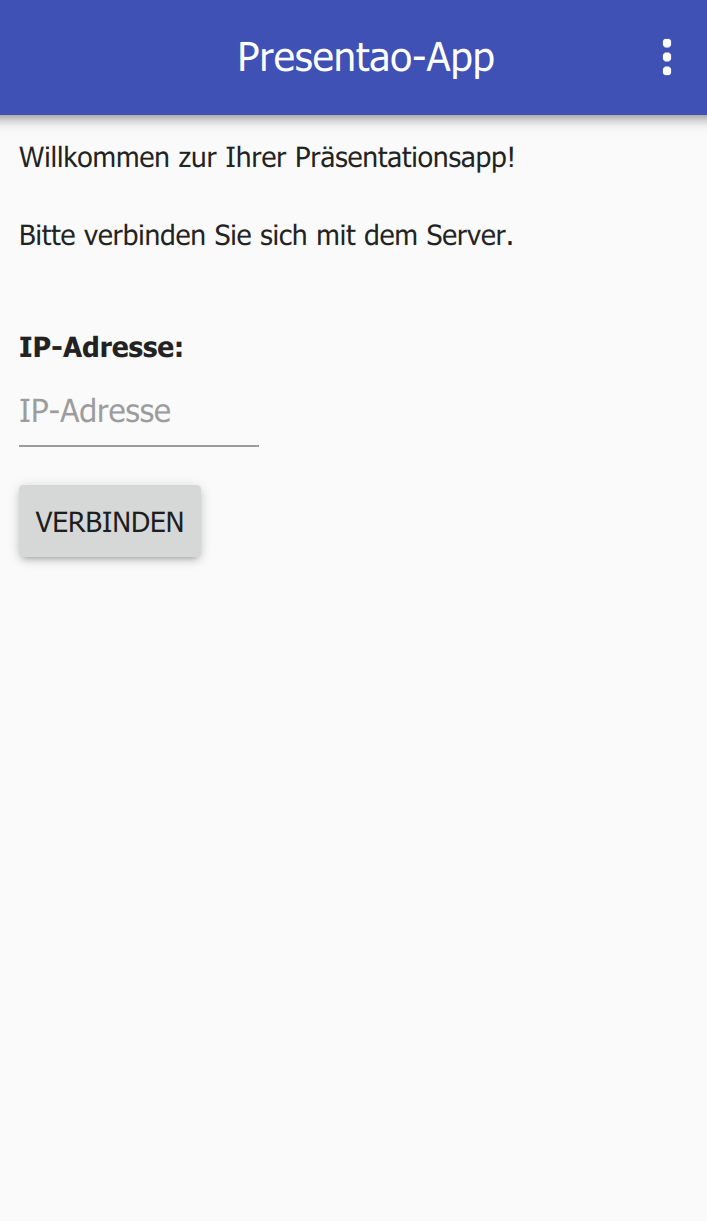
\includegraphics[scale=0.5]{GUI/Bilder/1-Startbildschirm.PNG}
	\end{minipage}
	%\hfill
	\begin{minipage}{0.31\linewidth}
		\centering
		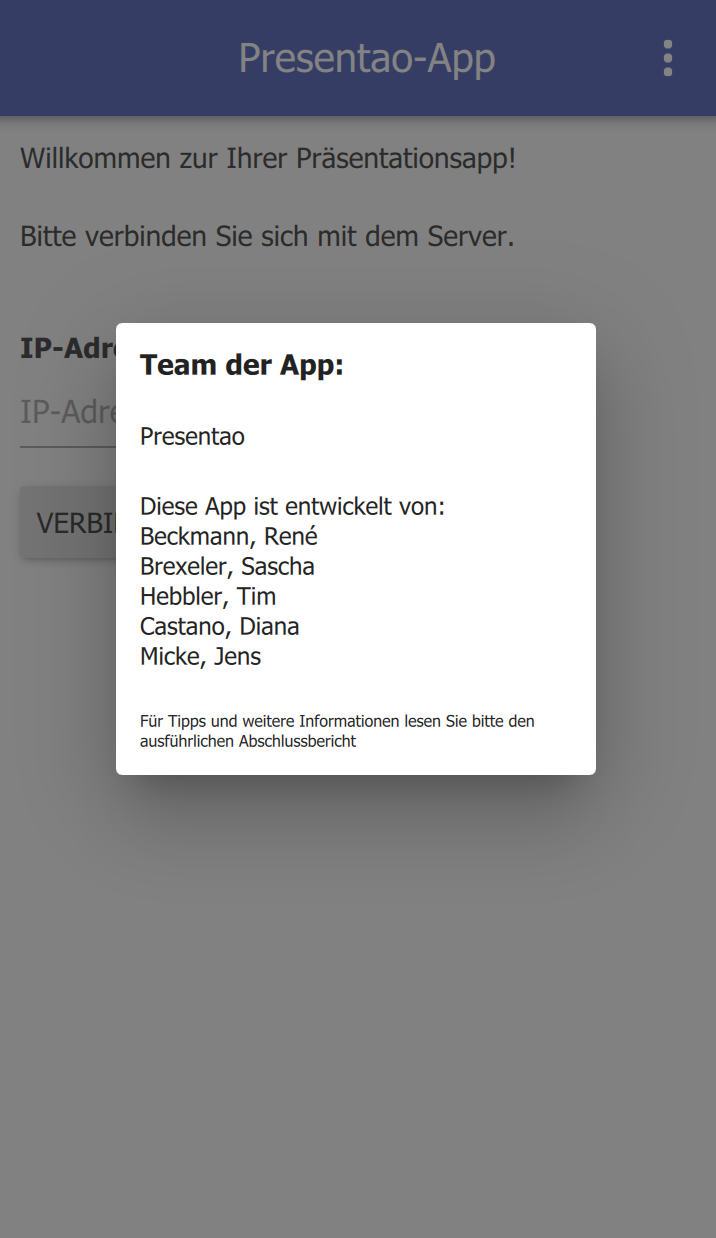
\includegraphics[scale=0.5]{GUI/Bilder/1-0-1-Startbildschirm-PopUP-Team.PNG}
	\end{minipage}
	\begin{minipage}{0.31\linewidth}
		\centering
		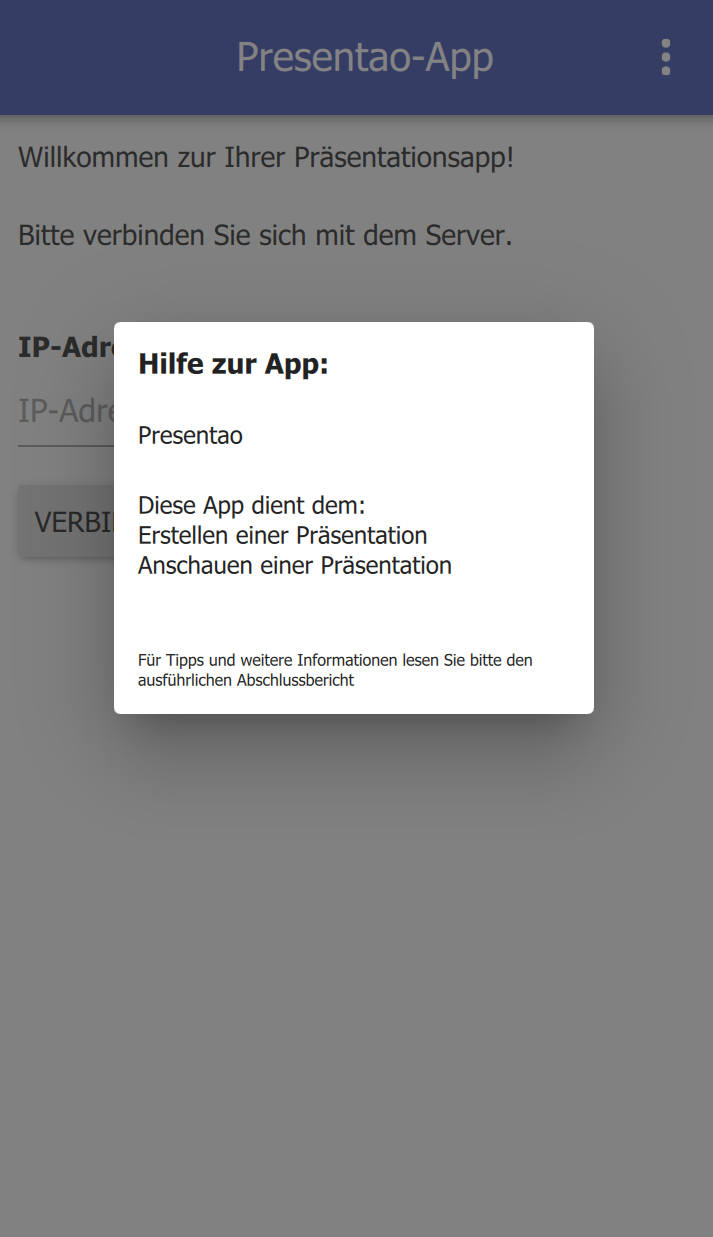
\includegraphics[scale=0.5]{GUI/Bilder/1-0-1-Startbildschirm-PopUP-Hilfe.PNG}
	\end{minipage}
	\caption{v.l.n.r.: Startbildschirm, Über die App, Hilfemenü{\tiny}}
	\label{client:Appstart}
\end{figure}

\newpage

\paragraph{Start der App}$\;$\\
Von dem Startbildschirm aus besteht die Möglichkeit, ein Menü (siehe \autoref{client:OptionsMenue}) durch Klicken auf den aus drei Punkten bestehenden Menü-Button (siehe \autoref{client:Appstart}) aufzurufen.
\\In diesem lassen sich zwei Pop-Ups zur Hilfe und zum Team aufrufen (siehe \autoref{client:Appstart}).
\begin{figure}[ht!]
	\centering
	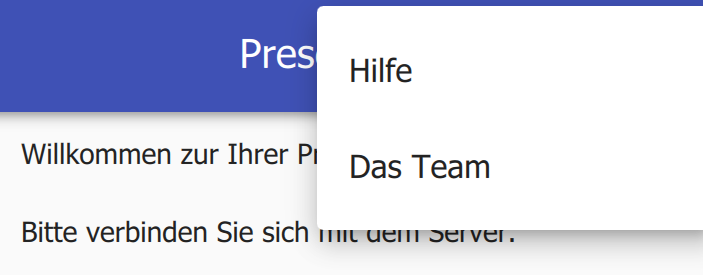
\includegraphics[scale=0.5]{GUI/Bilder/Info-Menu.PNG}
	\caption{Menü{\tiny}}
	\label{client:OptionsMenue}
\end{figure}
\paragraph{Verbindungsaufbau}$\;$\\
Des Weiteren kann der Benutzer nach Eingabe der gültigen IP-Adresse eine Verbindung zum Server als Zuhörer aufbauen. Die Eingabe der IP-Adresse erfolgt, wie in der dafür üblichen Notation, mit Punkttrennung. Eine Portangabe ist nicht nötig, da diese in Client und Server fest einprogrammiert ist.

\begin{figure}[ht!]
	\centering
	\begin{minipage}{0.31\linewidth}
		\centering
		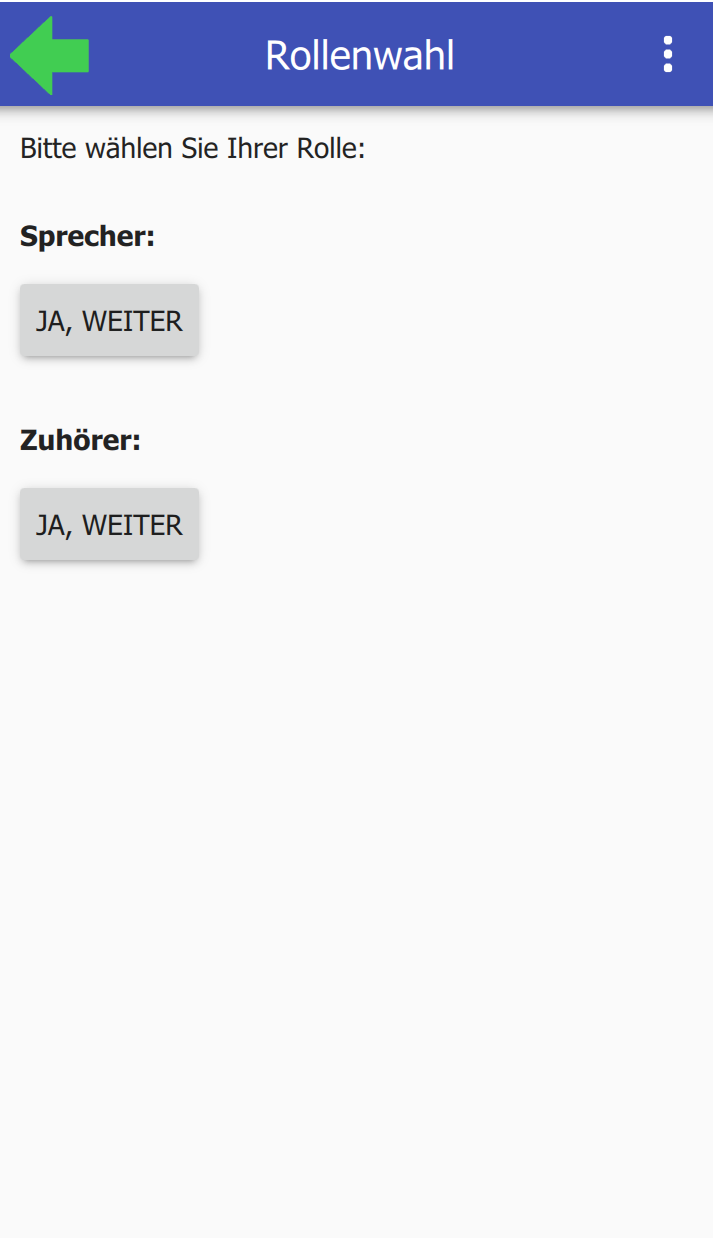
\includegraphics[scale=0.5]{GUI/Bilder/2-Rollenwahl.PNG}
	\end{minipage}
	%\hfill
	\begin{minipage}{0.31\linewidth}
		\centering
		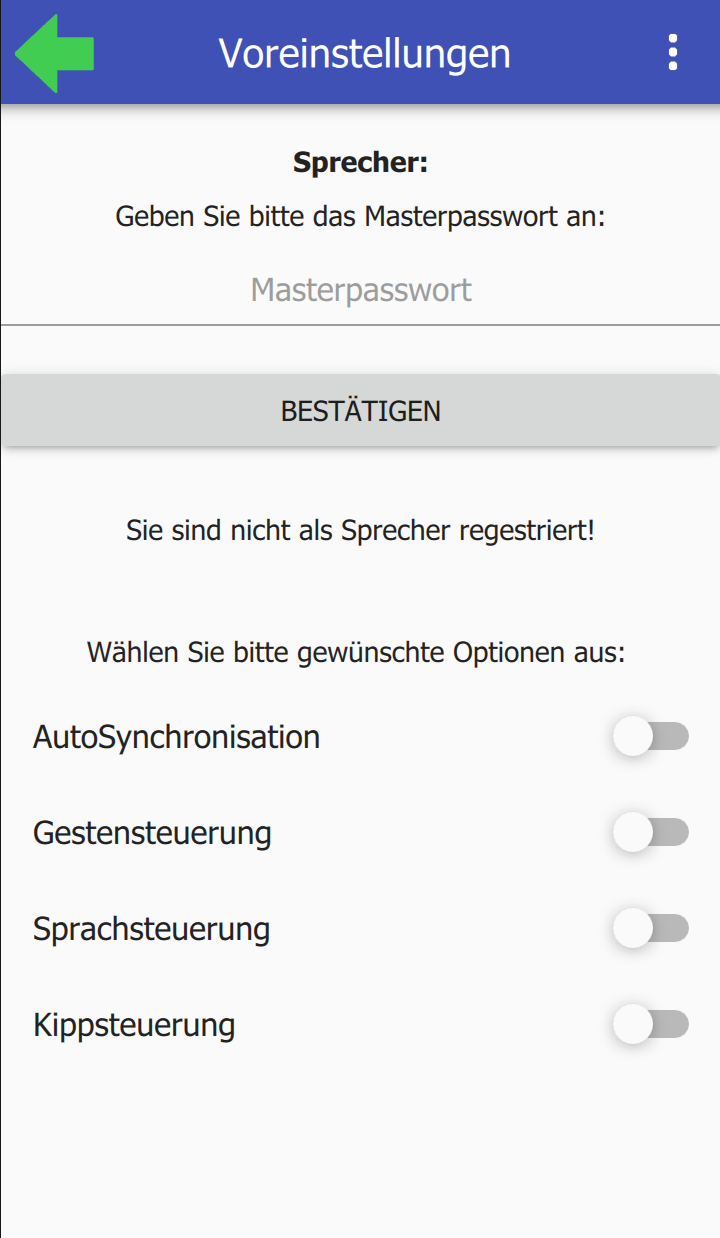
\includegraphics[scale=0.5]{GUI/Bilder/3-S-1-Voreinstellung.PNG}
	\end{minipage}
	\begin{minipage}{0.31\linewidth}
		\centering
		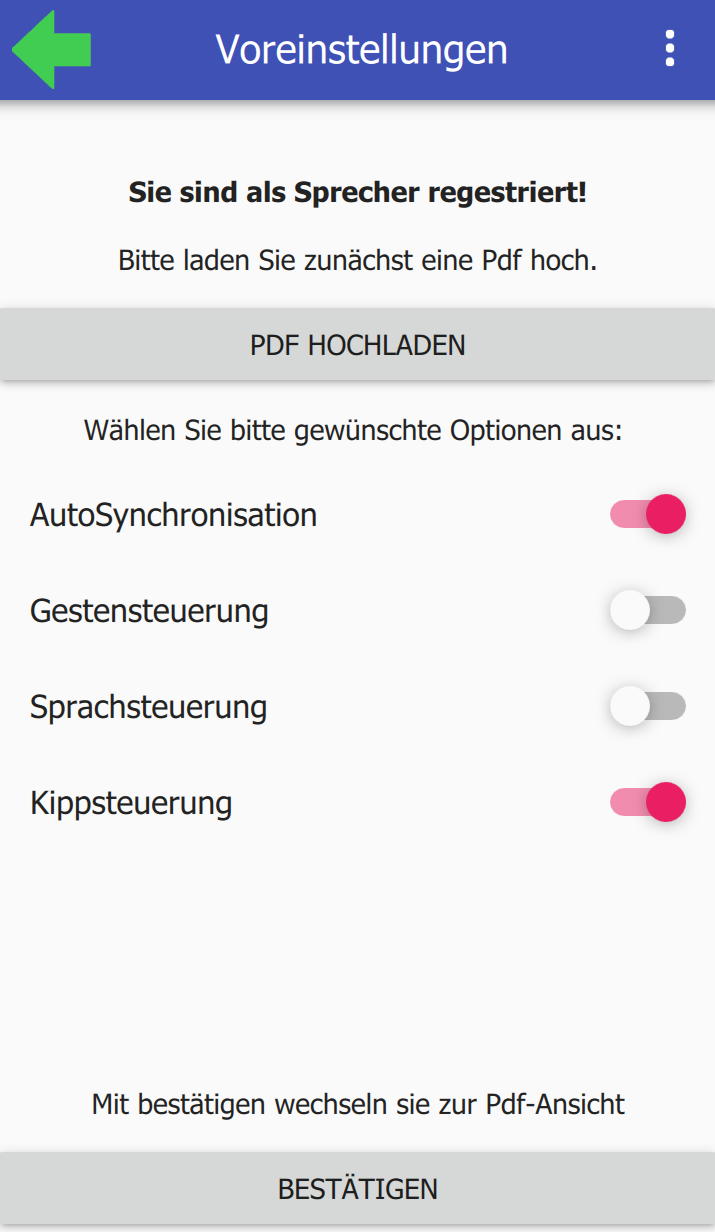
\includegraphics[scale=0.5]{GUI/Bilder/3-S-5-Voreinstellung.PNG}
	\end{minipage}
	\caption{v.l.n.r.: Rollenwahl, Voreinstellungen des Sprecher vor und nach Registrierung{\tiny}}
	\label{client:Rollenauswahl+S-Voreinstellungen}
\end{figure}

\newpage

\paragraph{Auswählen der eigenen Rolle}$\;$\\
Nach erfolgreichem Verbindungsaufbau wechselt die Ansicht in zur Rollenauswahl. Ein Label zeigt diese Position mittig der oberen Leiste (Toolbar) an (siehe \autoref{client:Rollenauswahl+S-Voreinstellungen}).
In dieser Toolbar befindet sich nun zusätzlich ein grüner nach links ausgerichteter Pfeil, um zur vorherigen Ansicht zu wechseln.
\\Die Rollenwahl ist wiederholbar und somit korrigierbar, aber unumgänglich implementiert, da weitere Einstellung und Möglichkeiten auf dieser Entscheidung aufbauen.
\paragraph{Voreinstellungen als Sprecher}$\;$\\
Der Sprecher muss sich zunächst als solcher bei dem Server registrieren. Dazu ist eine Passwortabfrage eingerichtet. Das sog. Masterpasswort ist "`mpw12345"'. Wenn die Eingabe fehlerhaft erfolgte, erscheint zusätzlich unter dem Textfeld zur Passworteingabe (siehe \autoref{client:Rollenauswahl+S-Voreinstellungen}) in Dickschrift der Hinweis: "`Bitte überprüfen Sie Ihre Passworteingabe"'. Sobald die korrekter Eingabe bestätigt ist, kann der Benutzer eine Pdf-Datei hochladen. Dazu muss der Nutzer eine Pdf-Datei über den File-Dialog (siehe \autoref{client:FileDialog}) suchen und auswählen. Der Client sendet die Pdf nach dem Öffnen an den Server, der diese direkt auf Seite 0 über den Projektor ausgibt. Bevor der Sprecher mit Bestätigen zur Pdf-Ansicht wechselt, sieht dieser noch eine Liste (ListView) mit einigen Optionen, aus denen er die Gewünschten über Schiebeschalter (SwitchDelegates) auswählen kann. Mit dem grünen Pfeil wechselt die Ansicht diesmal zurück zur Rollenwahl.

\begin{figure}[ht!]
	\centering
	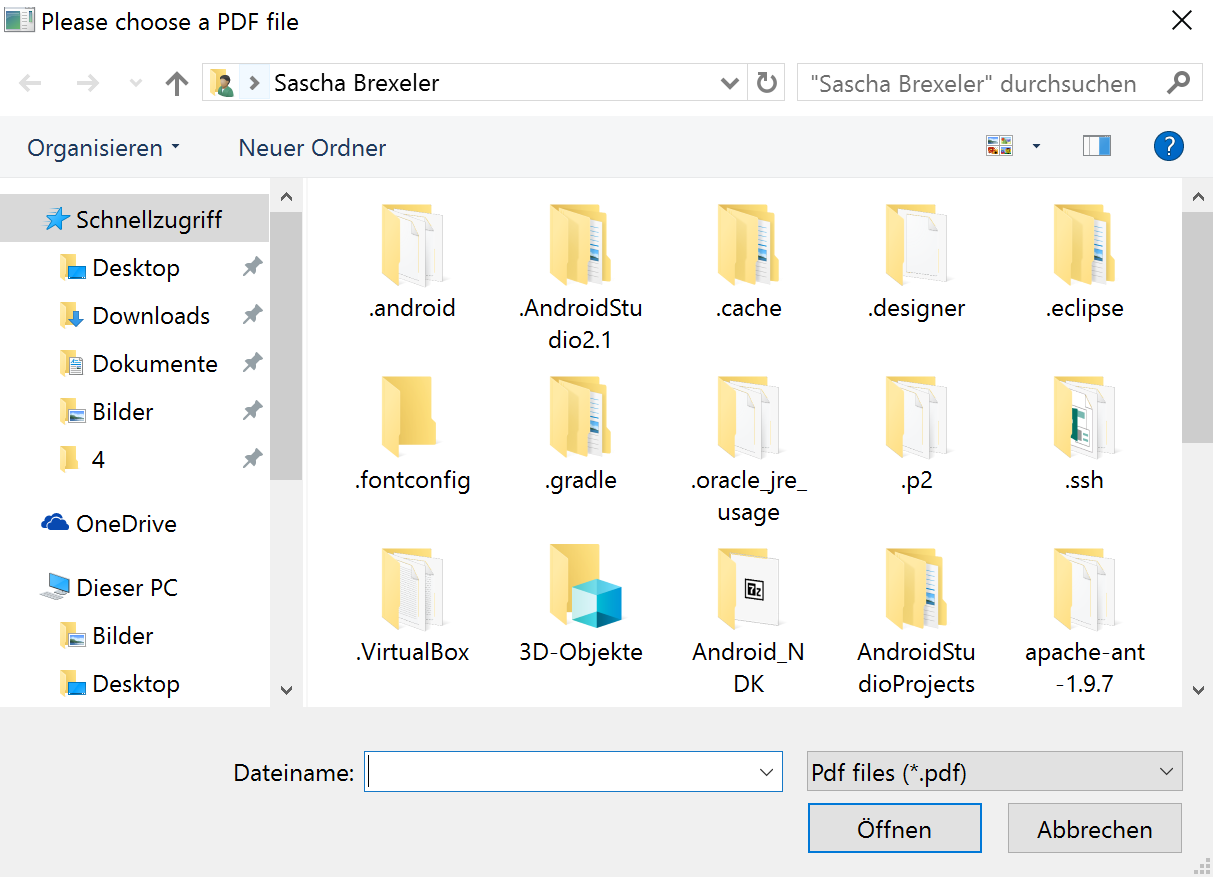
\includegraphics[scale=0.7]{GUI/Bilder/3-S-4-Voreinstellung.PNG}
	\caption{File-Dialog{\tiny}}
	\label{client:FileDialog}
\end{figure}

\newpage

\begin{figure}[ht!]
	\centering
	\begin{minipage}{0.31\linewidth}
		\centering
		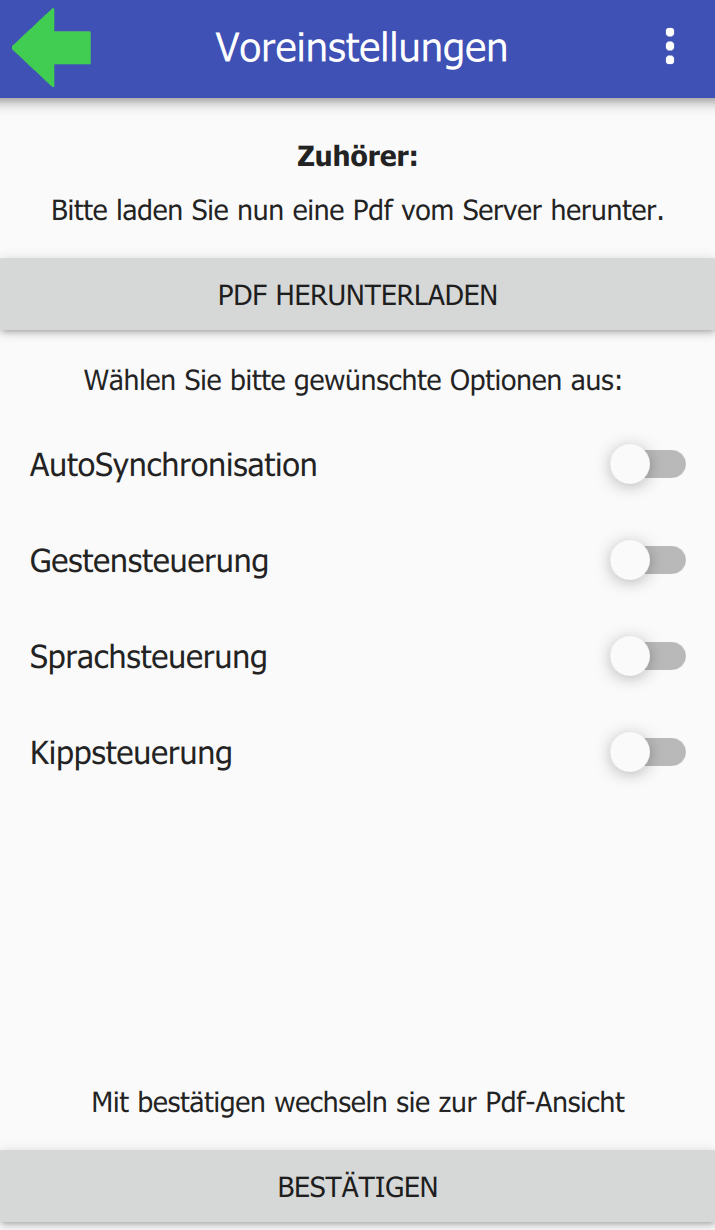
\includegraphics[scale=0.5]{GUI/Bilder/7-H-Voreinstellungen.PNG}
	\end{minipage}
	%\hfill
	\begin{minipage}{0.31\linewidth}
		\centering
		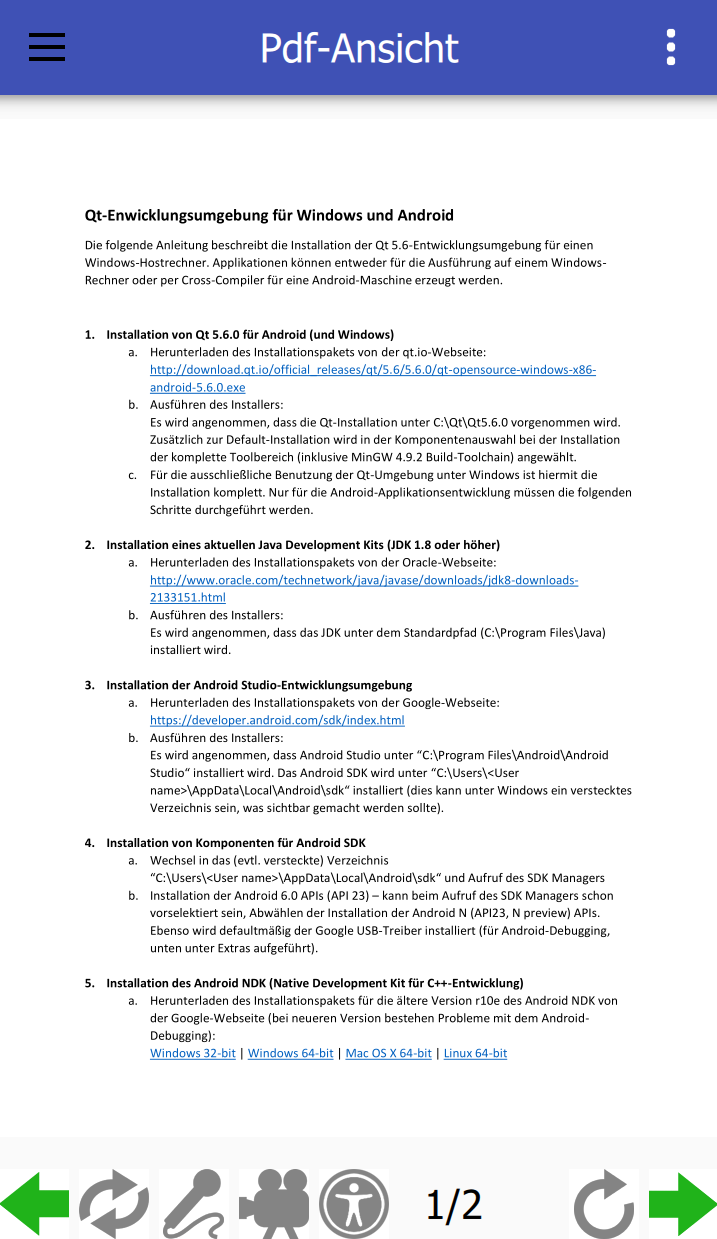
\includegraphics[scale=0.5]{GUI/Bilder/4-S-PDF-Ansicht.PNG}
	\end{minipage}
	\begin{minipage}{0.31\linewidth}
		\centering
		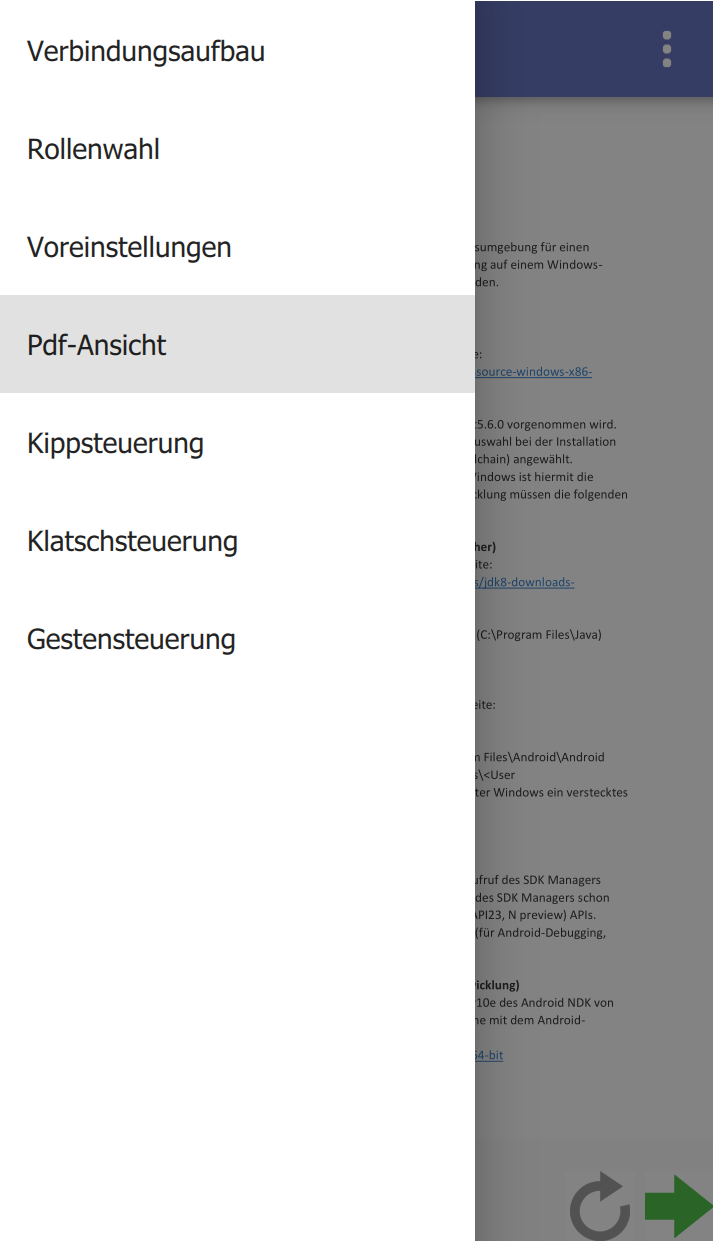
\includegraphics[scale=0.5]{GUI/Bilder/6-Menu-Button-Drawer-mit-Listview.PNG}
	\end{minipage}
	\caption{v.l.n.r.: Voreinstellungen des Zuhörers, PdfAnsicht und Drawer{\tiny}}
	\label{client:H-VoreinstellungenPdfAnsichtDrawer}
\end{figure}

\paragraph{Voreinstellungen als Zuhörer}$\;$\\
Als Zuhörer sind die Voreinstellungen ähnlich, jedoch entfällt die Passworteingabe und das Herunterladen einer Pdf-Datei ersetzt den Vorgang des Hochladens (siehe \autoref{client:H-VoreinstellungenPdfAnsichtDrawer}). Hierbei erfolgt (ohne eine Auswahlmöglichkeit) das Herunterladen der zuletzt auf dem Server geladenen Datei.
\paragraph{Pdf-Ansicht}$\;$\\
Bestätigen der Voreinstellungen des Sprechers oder Zuhörers bedingt einen Kontextwechsel zur Pdf-Ansicht (siehe \autoref{client:H-VoreinstellungenPdfAnsichtDrawer}).
\paragraph{Drawer}$\;$\\
Mit dem Wechsel zur Pdf-Ansicht ist der grüne Pfeil oben links durch einen weiteren aus drei waagerechten Strichen bestehenden Menü-Button ersetzt. Dieser Button öffnet eine vertikale Leiste (Drawer) am linken Bildschirmrand, welche ein ListView beinhaltet. Dieses ListView ermöglicht schnelle Navigation zu allen bisherigen Ansichten und Weiteren (siehe \autoref{client:H-VoreinstellungenPdfAnsichtDrawer}). Durch Wischen vom linken Bildschirmrand nach rechts lässt sich dieser ebenfalls einblenden. Die Navigation über das ListView im Drawer ist nur möglich, solange man nicht zu vorherigen Ansichten wechselt.

\begin{figure}[ht!]
	\centering
	
\includegraphics[scale=0.5]{GUI/Bilder/SchnellLeiste.PNG}
	\caption{Symbolleiste{\tiny}}
	\label{client:Symbolleiste}
\end{figure}

\paragraph{Symbolleiste}$\;$\\
Die Pdf-Ansicht beinhaltet eine Symbolleiste (siehe \autoref{client:Symbolleiste}) als Reihe von Icons am unteren Bildschirmrand. Mit ihr ist durch die Pfeile außen ein Blättern in der Pdf möglich. Intuitiv  kann der Benutzer durch Betätigen des linken Pfeils zurück blättern und mit dem Rechten vorwärts. Die anderen Buttons dienen zur Aktivierung/Deaktivierung von Bedienoptionen. Grün signalisiert hierbei den Status aktiviert und grau deaktiviert. Das Mikrofon steht für die Audiosteuerung, das Kamerasymbol für  Gestensteuerung und das Männchen mit den ausgestreckten Armen und Beinen im Kreis für die Kippsteurung. Neben diesem Symbol steht die Seitennummer der angezeigten Seite.
\\Die ineinander greifenden Pfeile signalisieren bei grün, dass die Autosynchronisation aktiv ist. Sobald diese nicht aktiv ist, erscheint ein weiterer Pfeil geschlungen im Uhrzeigersinn in grau auf der Symbolleiste links neben dem Pfeil. Die Funktion ist das manuelle Aktualisieren der Seitenzahl. Ein Sprecher sendet mit dem Refresh-Button die Seitenzahl, die auf seinem Device aktuell ist, zum Server, welcher sie an die Zuhörer-Clients weiterleitet. Ist als Sprecher der Status Autosynchronisation aktiviert, geschieht diese bei jedem Blättern automatisch. Zuhörer können über den Refresh-Button die aktuelle Seite manuell anfragen oder mit Autosynchronisation alle 2 Sekunden zu der aktuellen Seite zurück springen. Wenn der Sprecher blättert, erhalten die Zuhörer jedoch in jedem Fall die aktuelle Seite.

\paragraph{Informationen zur Benutzung}$\;$\\
Da das bisherige Hilfe-Pop-Up nur recht allgemeine Informationen enthält, sowie für weitere Hilfestellung auf diese eventuell nicht zur Hand liegenden Dokumentation verweist, kann sich der Benutzer über den Drawer zu einer Erklärung der Bedienmöglichkeiten navigieren. Diese Möglichkeit soll einen möglichst einfachen Einstieg ohne viel Ausprobieren sicherstellen und Anwendungsfehler verhindern. Um einen mit dieser Anwendung vertrauten Anwender nicht nach jedem Start durch diese Informationen zu führen, ist das Aufrufen optional (siehe \autoref{client:InformationenBedienhilfen}).

\newpage

\stepcounter{footnote}           % Fußnotenzähler weitersetzen          
\footnotetext{Text zur Kippsteuerung von Jens Helge Micke} 

\begin{figure}[ht!]
	\centering
	\begin{minipage}{0.31\linewidth}
		\centering
		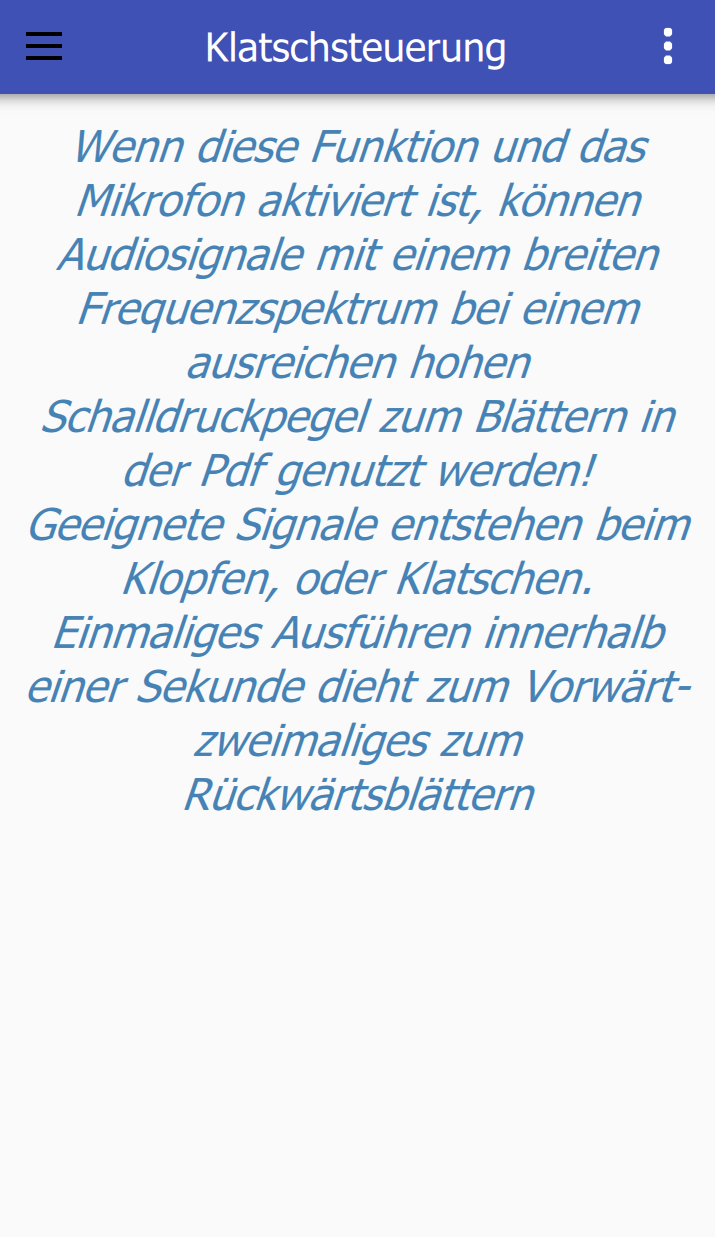
\includegraphics[scale=0.5]{GUI/Bilder/Klatschsteuerung.PNG}
	\end{minipage}
	%\hfill
	\begin{minipage}{0.31\linewidth}
		\centering
		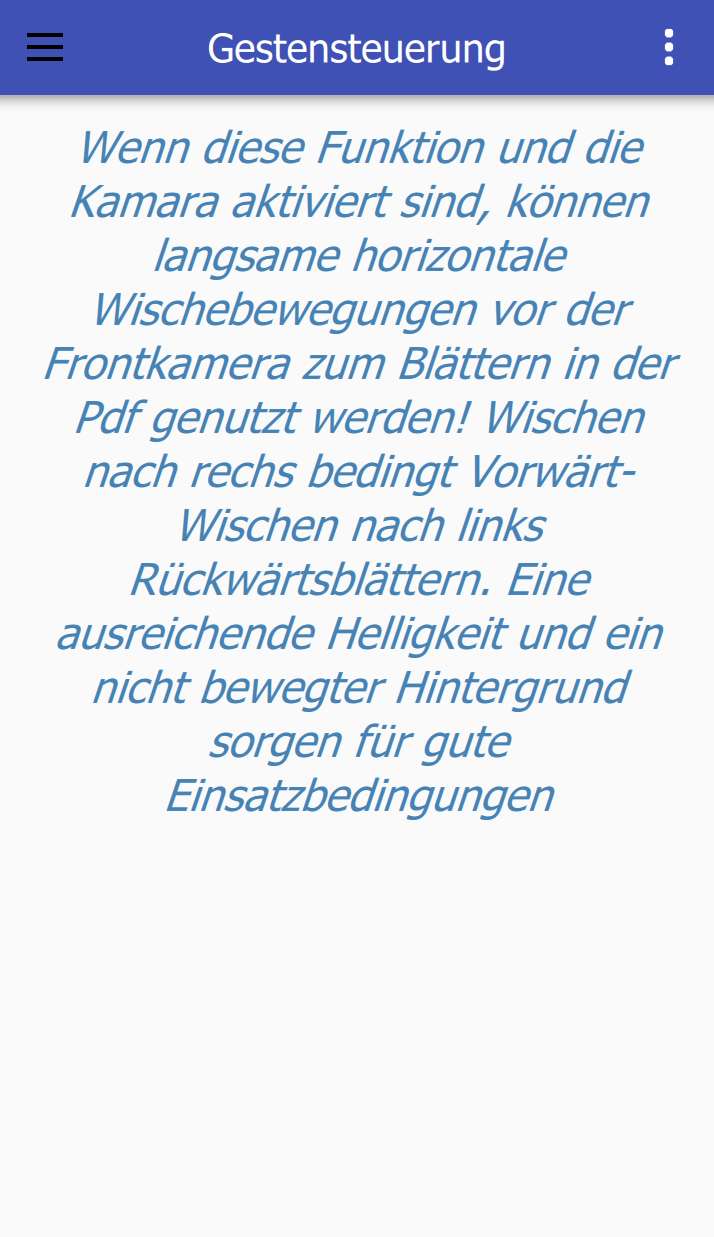
\includegraphics[scale=0.5]{GUI/Bilder/Gestensteuerung.PNG}
	\end{minipage}
	\begin{minipage}{0.31\linewidth}
		\centering
		
\includegraphics[scale=0.5]{GUI/Bilder/Kippsteuerung.PNG}
	\end{minipage}
	\caption[v.l.n.r.: Klatschsteuerung, Gestensteuerung und Kippsteuerung]{v.l.n.r.: Klatschsteuerung, Gestensteuerung und Kippsteuerung.\footnotemark}
	\label{client:InformationenBedienhilfen}
\end{figure}

\section[Serveranbindung]{Serveranbindung\footnote{Sascha Brexeler}}
\label{client-Serveranbindung}
Die Einbindung der Funktionsblöcke zur Kommunikation des Clients mit dem Server ist in Zusammenarbeit\footnote{zwischen Sascha Brexeler und René Beckmann} im Team entstanden. Details zur Kommunikation finden Sie in Kapitel \ref{server}.


\section[Software]{Software\footnote{Sascha Brexeler}}
\label{guiSoftware}
Die Software der GUI finden Sie im Git Repository \footnote{https://github.com/BeckmaR/EmbeddedMultimediaSS2016/tree/master/src/app\textunderscore gui}. Einige Funktionalitäten/Bibliotheken sind jedoch aus benachbarten Ordnern eingebunden.

\paragraph{Konzept}$\;$\\
Zur Umsetzung von GUI, Serveranbinung und der Einbindung der erweiterten Navigationsmöglichkeiten dient Qt-Creator 4.0.2 als IDE. Qt-Creator ist wegen seiner Plattformunabhängigkeit und der grafischen Beschreibungssprache qml für das den Client besonders geeignet. Programmiert ist die GUI überwiegend mit qml. Eine Kombination mit C++ Funktionen sowie das Signal-Slot-Prinzip kommen dabei an vielen stellen z.B. der Serveranbindung zum Einsatz. Mit dem Design-Tool von Qt-Creator stand eine graphische Programmiermöglichkeit von qml-Code zur Verfügung. Dieses stellt eine interessante Ergänzung zum "`schriftlichen"' Programmieren dar. Nach einer erfolgreichen Erprobung des Tools habe ich mich zugunsten der Homogenität des Codes gegen dieses entschieden.
\begin{figure}[ht!]
	\centering
	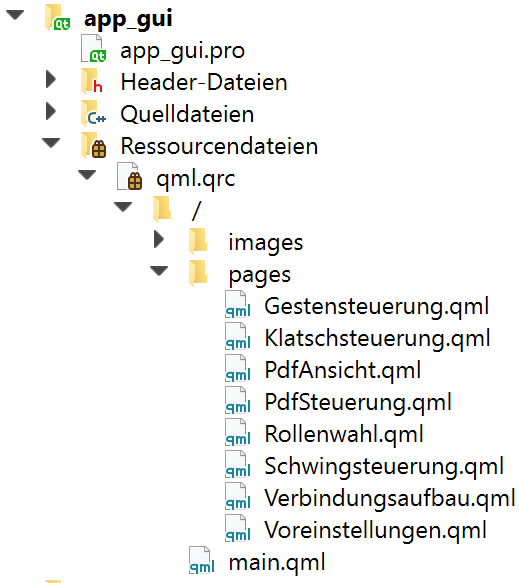
\includegraphics[scale=0.8]{GUI/Bilder/Projektordnerstruktur.PNG}
	\caption{Projektordnerstruktur {\tiny}}
	\label{client:Projektordnerstruktur}
\end{figure}


\paragraph{Struktur}$\;$\\
Der in Qt-Creator erstellte Projektordner app\textunderscore gui enthält die Projektdatei "`app\textunderscore gui.pro"', Header-Dateien, Quelldateien und Ressourcendateien (siehe \autoref{client:Projektordnerstruktur}). Unter den Quelldateien befindet sich das C++ Hauptprogramm "`main.cpp"'. Unter anderem instantiiert dieses beim Programmstart die Klasse QQmlApplicationEngine unter dem Namen engine. Im Anschluss daran öffnet die Methode engine.load(QUrl(QLatin1String("qrc:/main.qml"))) aus den Ressourcendateien das in qml geschriebene qml-Hauptprogramm "`main.qml"'. Die Datei qml.qrc verwaltet die Ressourcen. Dadurch ist es möglich aus dem qml-Hauptprogramm weitere Ressourcendateien z.B. in Form von Bildern oder weiteren in qml programmierten grafischen und funktionalen Elementen darzustellen oder aufzurufen, wenn diese sich in den Ressourcendateien befinden. Graphische Elemente können Rechtecke, Buttons, oder ganze Menüleisten sein und funktionale Elemente z.B. Timer.
Das StackView beinhaltet den Inhalt, welcher außerhalb der Randelemente Drawer oder ToolBar auf dem Bildschirm zur Anzeige kommt. Im Hauptprogramm befindet sich im StackView die Startansicht. Bei weiter Navigation durch die GUI ersetzen andere in qml geschriebene Dateien das StackView. Pop-ups überblenden es nur.
Für eine gute Übersicht über den Code bietet der Ct-Creator die Möglichkeit Codebl\"ocke einzuklappen(siehe \autoref{client:codeausschnitt-main.qml}).

\begin{figure}[ht!]
	\centering
	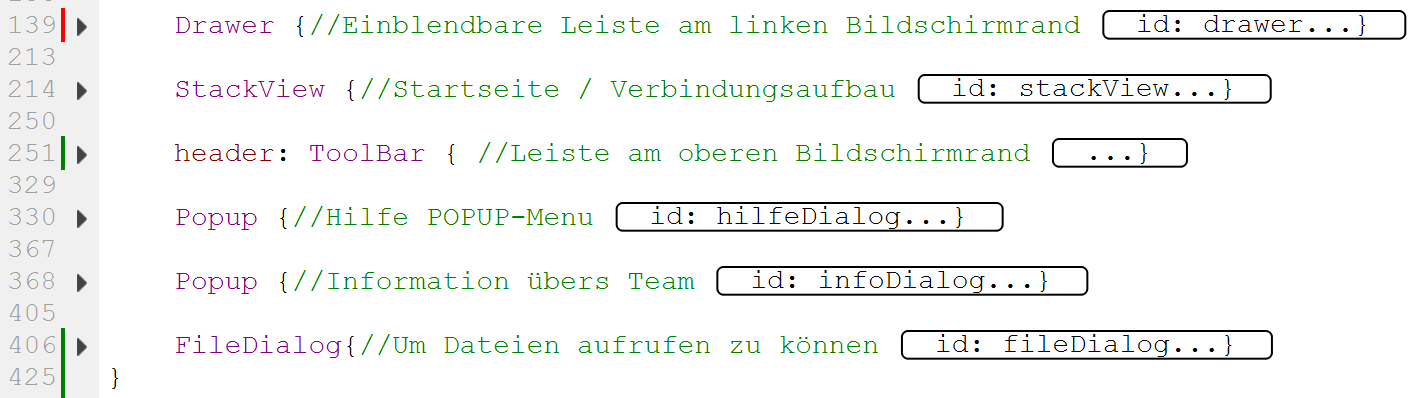
\includegraphics[scale=0.8]{GUI/Bilder/qml-main-Codeausschnitt.PNG}
	\caption{Wesentliche eingeklappte Codebl\"ocke des qml-Hauptprogramms "`main.qml"' {\tiny}}
	\label{client:codeausschnitt-main.qml}
\end{figure}

\paragraph{Zustandssteuerung}$\;$\\
Die Realisierung der grafischen Oberflächen entsprechend bisheriger Einstellungen ist über Zustände einer Variablen "`appState"' realisiert.Entsprechend der aktuellen Zustände sind Informationen mittels der Objekteigenschaft "`visible"' ein oder ausblendet oder über "`enable"' aktiviert oder deaktiviert. Außerdem gibt es weitere Variablen die speichern ob Einstellungen wie z.B. die automatische Synchronisation aktiviert ist, um vor dem ausführen von Funktionen zu überprüften ob diese gewünscht sind.

\newpage

\section{Navigation}
\subsection[Navigation mit dem Mikrofon]{Navigation mit dem Mikrofon\footnote{Diana Castano}}
\thispagestyle{fancy}

\subsubsection{Anforderungen}
Die Applikation setzte eine Navigation durch die PDF-Datei mithilfe des Mikrofons voraus, wodurch ein Klatschen oder Klopfen erkannt und als Blättern interpretiert werden konnte. Bei einmaligem oder zweimaligem Klatschen wurden entsprechende Signale zum vor- bzw. zurückblättern gesendet. \\
\\
Eine der Herausforderung dabei war, die Erkennung unabhängig von den äußeren Gegebenheiten erfolgen zu lassen (Raum mit oder ohne Nachhall). Außerdem sollte kein Signal zum Weiterschalten der Folien erzeugt werden, wenn ein starker Klang oder Ton aufgenommen wurde (z.B. wenn der Präsentator ggf. lauter sprechen musste). Der Algorithmus und die dabei berechneten Parameter sollten dabei nicht für jedes Gerät angepasst werden, selbst wenn die Mikrofone über unterschiedliche Eigenschaften verfügten. 

\subsubsection{Umsetzung}
Als erste Implementierung wurde eine Erkennung im Zeitbereich gewählt. Es wurde schnell festgestellt, dass dies eine sehr leise Umgebung voraussetzte. Selbst der Sprecher konnte das Signal aktivieren, wenn er sehr nah am Mikrofon war. Aus diesem Grund erfolgte die Erkennung im Frequenzbereich. Die Signalverarbeitung war hierbei aufwändiger, allerdings wurden damit die Herausforderungen überwunden.\\
\\
Das Modul  \href{http://doc.qt.io/qt-5/qtmultimedia-index.html}{Qt Multimedia 5.7} stellt verschiedene C++ Klassen zur Verfügung, die für die Steuerung des Mikrofons hilfreich sind. Eine Abfrage über die verfügbaren Aufnahmegeräte konnte mit \textit{QAudioDeviceInfo} durchgeführt werden. Das Audio-Format und die Darstellung der Daten wurden mithilfe der Klasse \textit{QAudioFormat} festgelegt. Folgende Einstellungen wurden verwendet:

\begin{center}
	\begin{itemize}
		\item Abtastrate: 8 kHz
		\item Anzahl der Kanäle: 1 (mono)
		\item Bytes pro Abtastwert: 2
		\item Format der Abtastwerte: Signed Integer
		\item Byte-Reihenfolge: Little Endian
		\item Codec: Linear PCM	
	\end{itemize}
\end{center}

Die Klasse \textit{QAudioInput} bietet eine Schnittstelle um akustische Signale aus einem Mikrofon aufzunehmen. Dafür muss zuerst ein Aufnahmegerät mithilfe von \textit{QIODevice} im Lesemodus zum Empfangen der Daten geöffnet werden. Jede Sekunde werden neue Daten aus dem Mikrofon gelesen. Die Daten, die sich im Buffer befindet werden zuerst in einem \textit{QByteArray} gespeichert. Anschließend werden die Abtastwerte vom \textit{Signed Integer} Format zum \textit{Float} umgewandelt und in einem \textit{QVector} gespeichert, um eine Fourier-Analyse des Signals zu ermöglichen.\\
\\
Die Analyse im Frequenzbereich erfolgt durch das Spektrogramm, das eine Zusammensetzung des akustischen Signals in seinen einzelnen Frequenzen im zeitlichen Verlauf darstellt. Dafür müssen zuerst die im Buffer gespeicherten Abtastwerte in sich überlappende Rahmen aufgeteilt werden, wie in \autoref{fig:image0} dargestellt wird:

\begin{figure}[h]
	\centering
	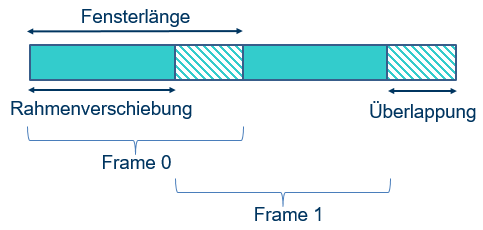
\includegraphics[width=1\textwidth]{beatcontrol/BeatBilder/bild0.png}
	\caption{Aufteilung des Signals in Rahmen}
	\label{fig:image0}
\end{figure}

Dafür wurden folgende Größen gewählt:
 
\begin{center}
	\begin{itemize}
		\item Länge des Buffers: 16000 Bytes
		\item Länge der einzelnen Rahmen: 256 Werte (circa 25 ms)
		\item Rahmenverschiebung: 80 Werte (10 ms)
		\item Überlappung: 176 Werte
		\item Anzahl von Rahmen: 98
		\item Fenstertyp: Hanning
	\end{itemize}
\end{center}


Falls das Signal sich nicht in genau dieser Anzahl von Rahmen aufteilen lässt, werden Nullen am Ende des Signals hinzugefügt. Da die Länge der Rahmen endlich ist und kein Vielfaches der Periode des Signals darstellt, müssen die Rahmen mit einer Fensterfunktion gewichtet werden, um den Leck-Effekt zu vermeiden.  \\
\\
Anschließend muss die Diskrete Fourier-Transformation (DFT) für jeden Rahmen berechnet werden. Die Schnelle-Fourier Transformation (FFT) ist ein effektiver Algorithmus zur Berechnung der DFT. Für die Implementierung der FFT in Qt 5.7 wurde die Open-Source Bibliothek \href{ http://ldesoras.free.fr/prod.html}{FFTReal} verwendet, die für schnelle Berechnungen optimiert ist (besonders wenn die Anzahl der FFT-Punkte schon bekannt ist). \\
\\
Es wurde zunächst der Betrag der Transformation berechnet, daraufhin erfolgte die Berechnung des Logarithmus. Folge dessen wurden die Ergebnisse in Form einer Matrix in einer CSV-Datei gespeichert. Die Spalten stellen die einzelnen Rahmen dar (Zeitindex), wobei die Reihen der Frequenzanteile (Frequenzindex) entsprechen. Anschließend wurde die Datei mit MATLAB gelesen und geplottet. \autoref{fig:image1} zeigt eine farbcodierte Darstellung dieser Matrix: \\

\begin{figure}[h]
	\centering
	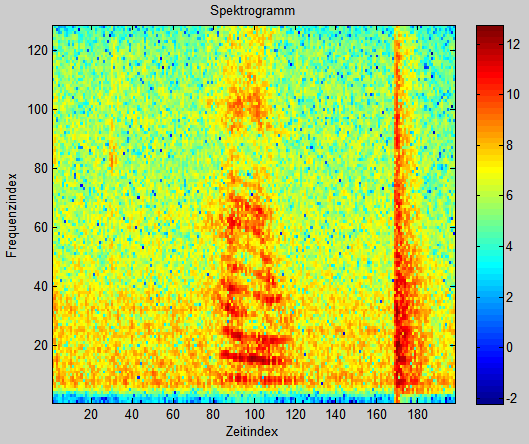
\includegraphics[width=1\textwidth]{beatcontrol/BeatBilder/bild1.png}
	\caption{Spektrogramm ("`Hallo"' $+$ Klatschen)}
	\label{fig:image1}
\end{figure}

Hier ist die zeitliche Entwicklung aller Frequenzkomponenten des Signals zu sehen. In diesem Fall wurde ein "`Hallo"' und folglich ein Klatschen aufgenommen. Dabei wird deutlich, dass ein Klatschen ein sehr breitbandiges Signal erzeugt, in welchem alle Frequenzen erhalten sind. Ein "`Hallo"' hingegen enthält nur bestimmte und wenige Frequenzanteile. Es wurde festgestellt, dass die Erkennung auf dieser Analyse erfolgen konnte. \\
\\
Der Algorithmus berechnet die Summe der Frequenzanteile jeder Rahmen, wie in \autoref{fig:image2} zu sehen ist (in diesem Fall wurden zwei Klatschen aufgenommen). Wenn die Summe eine bestimmte Schwelle überschreitet, und der darauffolgende Wert wiederum kleiner ist, wird dies als ein Klatschen erkannt. Anschließend wird für eine Sekunde ein Timer gestartet. Wenn innerhalb dieser Zeit die gleiche Erkennung erfolgt, wird das Signal zum Zurückblättern gesendet. Ansonsten wird das Signal zum Vorblättern gesendet.

\begin{figure}[h]
	\centering
	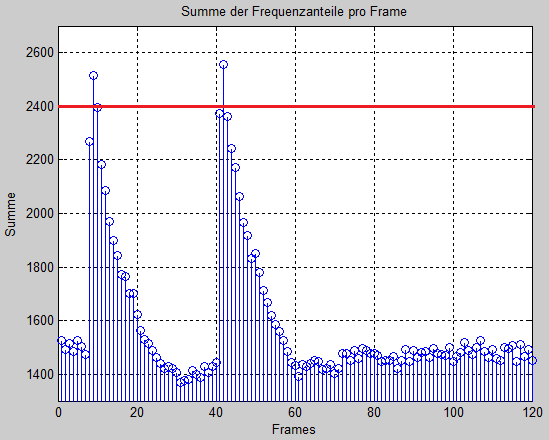
\includegraphics[width=1\textwidth]{beatcontrol/BeatBilder/bild2.png}
	\caption{Summe der Frequenzkomponenten}
	\label{fig:image2}
\end{figure}

\subsubsection{Erweiterungen}
Die Steuerung einer Präsentation mittels fließender Sprache ist nur mit umfangreichen Kenntnissen der Wahrscheinlichkeitsrechnung und der Signalverarbeitung möglich. Wenn man die begrenzte Zeit des Projektes in Betracht nimmt, wird schnell festgestellt, dass  eine umfangreiche Spracherkennung durch das Programm in der Kürze der Zeit nur schwer umgesetzt werden kann. Man könnte allerdings Open-Source Bibliotheken verwenden, die beispielsweise bereits ein Erkennungssystem für ein kleines Vokabular implementiert haben.\\
\\
Allerdings stellt die Applikation einen ersten wichtigen Schritt in diese Richtung dar. Für eine Erkennung im Frequenzbereich bildet das Spektrogramm den Ausgangspunkt für weitere Analysen des Signals. 


% !TeX encoding = UTF-8
\chapter{Gestensteuerung}
\thispagestyle{fancy}

Die Gestensteuerung hat die Aufgabe Handbewegungen über eine Smartphone-Kamera zu erkennen. Dabei werden zwei Richtungen erkannt und Signale zum vor- und zurückblättert von PDF-Seiten gesendet. Auf Grund der Vorlesung und Recherchen im Internet war schnell klar, dass \href{http://opencv.org/}{OpenCV} eine zweckmäßige Bibliothek darstellt. Als Qt Basis wurde die Version 5.7 und OpenCV in der Version 3.1 verwendet. Der Code für die Gestenerkennung befindet sich unter folgendem \href{https://github.com/BeckmaR/EmbeddedMultimediaSS2016/tree/master/src/handcontrol}{Link}. Hierbei wurde ein C++ Klasse "`handcontrol"' erstellt, welche in die App eingebunden ist.

\section{Auslesen von Videoframes aus einer Kamera}
Im Laufe des Projektes stellte sich heraus, dass die Einbindung der Kamera, auf den verschiedenen Plattformen Windows und Android, die größte Herausforderung darstellt. Die Windows Unterstützung wurde hauptsächlich ausgewählt, um den Algorithmus nicht umständlich auf einem Android Gerät jedes mal testen zu müssen. Die Implementierung auf der Windows-Plattform war relativ einfach, da OpenCV schon eine Funktion \href{http://docs.opencv.org/3.1.0/d8/dfe/classcv_1_1VideoCapture.html}{VideoCapture} bietet, welche einzelne Videoframes aus eine Kamera auslesen kann und diese in einer Matrix abspeichert. Diese Methode funktionierte leider nicht auf einen Android-Gerät. Hinweise: nachfolgende Funktionsweisen beziehen sich auf den Entwicklungsstand vom 20.7.2016, ggf. sind schon Bugs behoben oder neue Möglichkeiten zur Kameraauswertung hinzugekommen. Vom Autor wurden unterschiedlichste Varianten zum Auslesen der Kamera über mehrere Stunden untersucht. Von Qt werden hauptsächlich \href{http://doc.qt.io/qt-5/videooverview.html}{zwei Möglichkeiten} für das Auslesen eines VideoFrames angeboten. \href{http://doc.qt.io/qt-5/qabstractvideosurface.html}{QAbstractVideoSurface} definiert eine abstrakte C++ Klasse welche die Funktion present() beinhaltet, welcher die einzelnen Videoframes nacheinander übergeben werden. Ähnlich verhält es sich mit \href{http://doc.qt.io/qt-5/qvideoprobe.html}{QVideoProbe} wobei man hier die Verbindung über ein Connect() mit Signal und Slot hergestellt werden muss. Eine weitere Möglichkeit besteht seit Qt 5.5 darin, ein Video Filter\footnote{\label{video_filter}https://blog.qt.io/blog/2015/03/20/introducing-video-filters-in-qt-multimedia/} in QML zu verwenden und mit Hilfe der Klasse \href{http://doc.qt.io/qt-5/qabstractvideofilter.html}{QAbstractVideoFilter} die einzelnen Videoframes in C++ zu analysieren und ggf. wieder nach QML zu transformieren. Die C++ QCamera funktioniert nicht auf Android-Geräten (\href{https://bugreports.qt.io/browse/QTBUG-41194}{1},\href{http://stackoverflow.com/questions/28041741/qt-qml-camera-to-c-qimage-on-android}{2}), sodass auf das in QML integrierte Camera Objekt zurückgegriffen wird. Bei der QAbstractVideoFiler Variante konnten die Videodaten in Android nicht in den CPU-Adressraum gemappt werden. Mit QVideoProbe war dies möglich. Hierbei wird aus QML das QCamera Objekt in C++ adressierbar gemacht und mit dem QVideoProbe verbunden. Seit Qt 5.6 existiert ein VideoOutput Objekt in QML welches das Auslesen und Anzeigen von VideoFrames steuert, sodass das hier angegebene \href{http://stackoverflow.com/questions/28041741/qt-qml-camera-to-c-qimage-on-android/33238150\#33238150}{Beispiel} noch um ein VideoOutput Objekt ergänzt werden muss. Um keine größeren Unterschiede zwischen dem Algorithmus für die Windows- und der Androidversion zu haben, ist es wünschenswert beide Cameras über Qt auslesen zu lassen. Leider funktioniert der oben für Android vorgestellte Ansatz für Windows nicht. Hier ist ein Workaround mit einer C++ QCamera und dem QAbstractVideoSurface nötig, um ein QVideoFrame zu erhalten. Die neue Variante mit dem "`Video Filter"' wurde auch untersucht, hat aber nur auf ein paar Androidgeräten funktioniert \href{https://bugreports.qt.io/browse/QTBUG-47934/}{QTBUG-47934}. Anscheinend gibt es dort noch Fehler in dem Qt-Framework. Unter folgendem \href{https://wiki.qt.io/Qt_5.7_Multimedia_Backends}{Link} gibt es eine Auflistung welche Funktionen in dem Qt-Multimedia-Framework-5.7 auf den verschiedenen Plattformen aktuell funktionieren.

\subsection{Verbesserungen}
Die mit Qt 5.5 eingeführten Video Filter scheinen ein gute Weg zu sein, um VideoFrames in Qt analysieren zu können. Leider ist aktuell die Implementierung nicht auf allen Androidgeräten funktional, sodass auf ein Workaround mit QVideoProbe zurückgegriffen werden musste. Diese Variante ist aber leider nicht optimal, da sie Verzögerungen zwischen dem Aufnehmen und dem Aufruf der Funktion present() enthält\footnote{https://blog.qt.io/blog/2015/03/20/introducing-video-filters-in-qt-multimedia/\#comment-1195419}. Eine weitere Möglichkeit besteht, QML \href{http://doc.qt.io/qt-5/qml-qtquick-shadereffect.html}{ShaderEffect} mit OpenGL zu verwenden. Da die Android Kamera seine Videoframes auf der Grafikkarte in OpenGL Texture vorhält \footnote{https://blog.qt.io/blog/2015/03/20/introducing-video-filters-in-qt-multimedia/\#comment-1195414}, wäre es sinnvoll diese auch dort weiter zu verarbeiten. Das kann seit neuem mit Video Shader Objekten direkt in QML programmiert werden. Außerdem war es dem Autor über QML nicht möglich exakte Auflösungen und Frameraten einzustellen. Anscheinend ignoriert Qt gewisse Parameter auf verschiedenen Platformen oder es stehen nicht alle Einstellung zur Verfügung. Jedenfalls sind diese nicht richtig dokumentiert. Ein Problem ist außerdem, dass es vorkommen kann das Frameraten von 30 fps auf 16 fps einbrechen oder kein reproduzierbares Verhalten zeigen. Dieser Punkt konnte innerhalb der Arbeit leider nicht geklärt werden. Eine andere Möglichkeit, welche nicht weiter verfolgt wurde, wäre über Qt mit den \href{http://doc.qt.io/qt-5/qtandroidextras-module.html}{Qt Android Extras} die Androidkamera über Java Code in die Qt Anwendung einzubetten, ggf. auch über das vorhandene OpenCV Java Binding. 

\section{Handerkennungsalgorithmus}
Aus Qt liegen die QVideoFrames als RGB (Windows) und als YUV420 (Android) vor. Diese werden als erstes in Grauwertbilder umgewandelt. Bei dem Android QVideoFrame muss keine pixelweise Konvertierung durchgeführt werden, sondern es wird nur der Luminanz Y Teil des Bildes genommen. Anschließend wird das Differenzbild zwischen dem aktuellen und vorherigen Grauwertbild berechnet. Hierbei achtet OpenCV selbständig darauf, dass eine Sättigung im Zahlenbereich durchgeführt wird.

\begin{figure}[ht!]
\centering
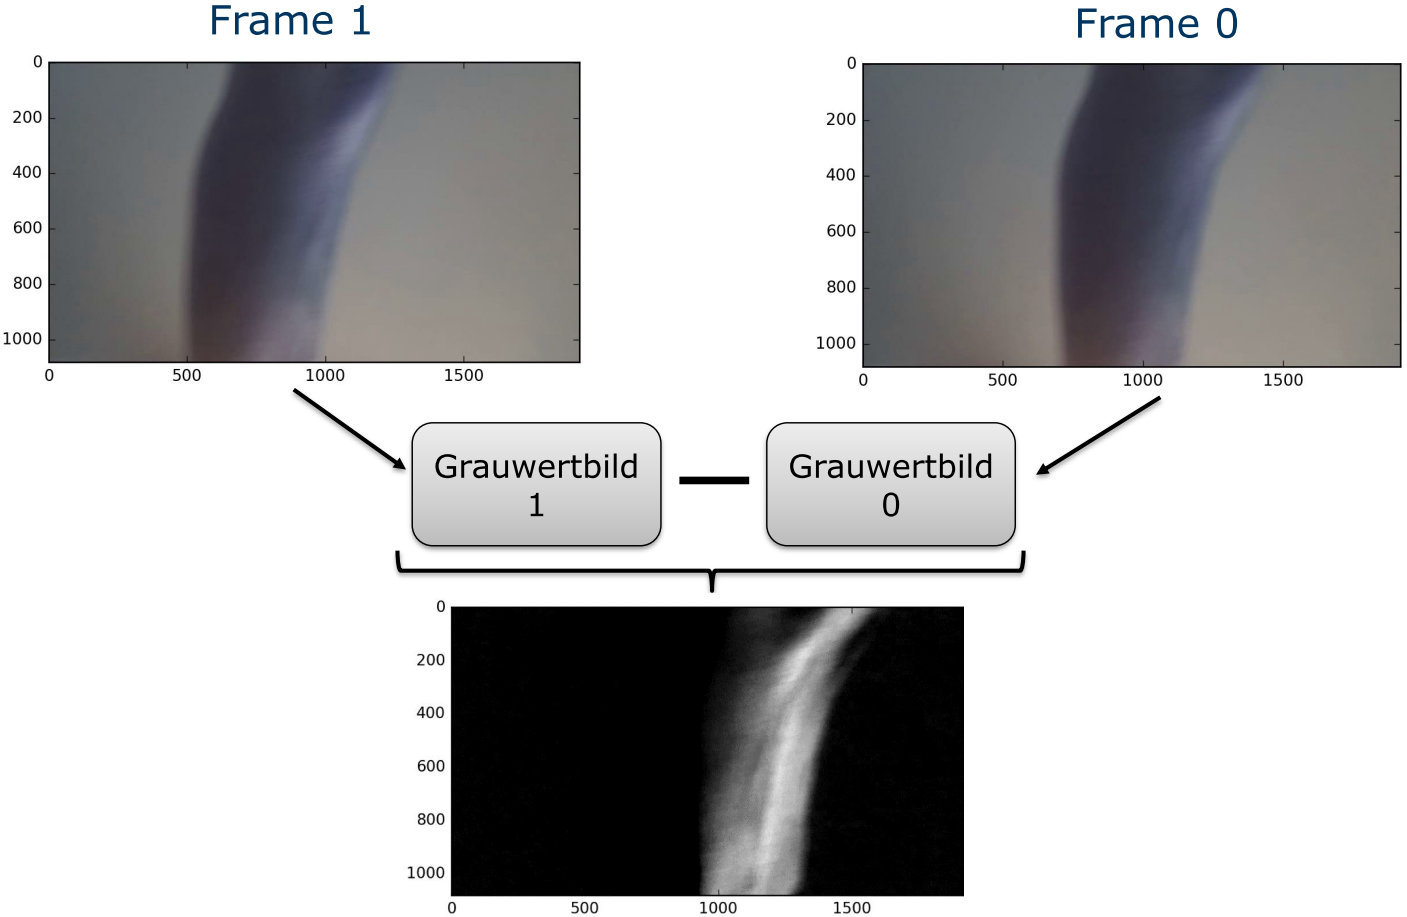
\includegraphics[angle=0,width=14cm]{handcontrol/Bilder/diff_frame1-frame0.png}
\caption{Differenzberechnung zwischen aktuellem und vorherigen Grauwertbild}
\end{figure}

Im nachfolgenden Schritt wir mit Hilfe der reduce() Funktion von OpenCV ein Mittelwert über alle Spalten gebildet. Man erhält einen Zeilenvektor wobei jeder Eintrag den Mittelwert eine Spalte repräsentiert. Hierbei kann man schnell erkennen wo sich in der Horizontalen die größten Änderungen ergeben. Das nennt der Autor Histogramm, da es die Häufigkeitsverteilung darstellt.

\begin{figure}[ht!]
\centering
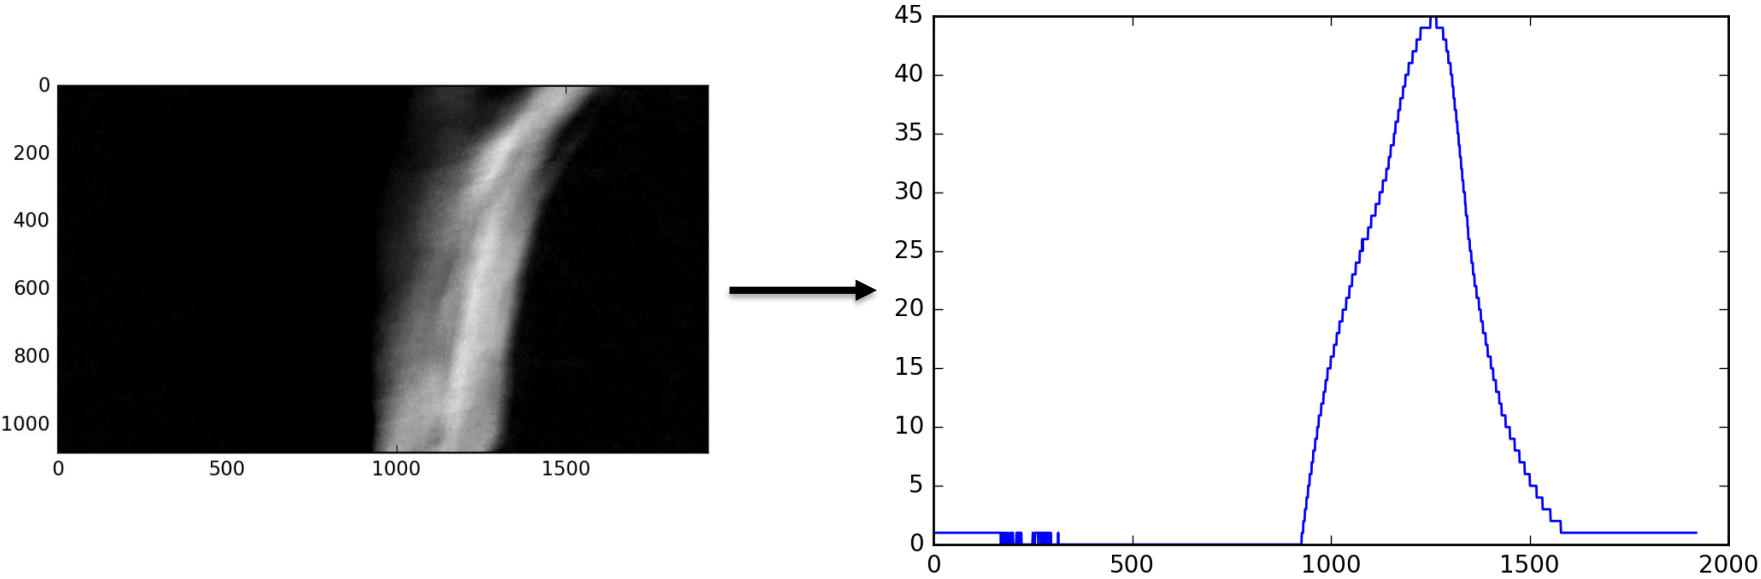
\includegraphics[angle=0,width=14cm]{handcontrol/Bilder/diff_frame_to_hist.png}
\caption{Berechnung des Histogramms über die Spalten eines Differenzbildes}
\end{figure}

Untersucht man die Verschiebung des Histogramms über die Horizontalen, kann man Handbewegungen erkennen. Hierbei wird als erstes der Schwerpunkt des Histogramms gebildet. Das geschieht mit Hilfe einer kumulierten Summe über alle Histogrammwerte. Würde man nur den maximalen Wert des Histogramms betrachten, kann bei verrauschten Bildern eine zu große Abweichung auftreten. Vor dem Berechnen des Schwerpunktes wird noch ein konstanter Faktor subtrahiert, um den ggf. existierenden Rauschteppich zu entfernen. Zur weiteren Fehlerreduktion wurden im folgenden nur diese Schwerpunkte ausgewählt, welche auch mindestens einen gewissen maximalen Histogrammwert aufweisen. Der Wert kann im Sourcecode nachgelesen werden. Um auszuwerten, ob eine PDF vor- oder zurückgeblättert werden soll, untersucht der Algorithmus zeitlich aufeinanderfolgende Schwerpunkte von Histogrammen der Differenzbilder. Er sendet ein Signal, wenn ohne Unterbrechung der Schwerpunkt eine gewisse Zeit in eine der beiden Richtungen gewandert ist. Um den GUI-Thread nicht zu überlasten und um eine flüssige Bedienung der GUI sicher zu stellen, wurde der Algorithmus in ein QThread verschoben. Der so beschriebene Algorithmus benötigt mit 30 Frames pro Sekunde auf Windows ~7ms und auf Android ~10 ms. Somit ist die Echtzeitfähigkeit gegeben. Als Alternative zum dem Differenzbild wurde auch der in OpenCV implementierte Background Substraction Algorithmus (\href{http://docs.opencv.org/3.0-rc1/d7/d7b/classcv_1_1BackgroundSubtractorMOG2.html}{BackgroundSubtractorMOG2}) untersucht. Dieser schätzt den Hintergrund über gaußsche Mischungsverhältnisse mit Mittelwert und Kovarianzmatrix. Leider benötigt der Algorithmus viel Berechnungszeit (~14 Windows und ~30 ms Android) und kratzt somit bei Android Geräten an der Echtzeitfähigkeit. Außerdem würde eine solche Implementierung zu viel Energie des Akkus verbrauchen und wurde deshalb verworfen.

\begin{figure}[ht!]
\centering
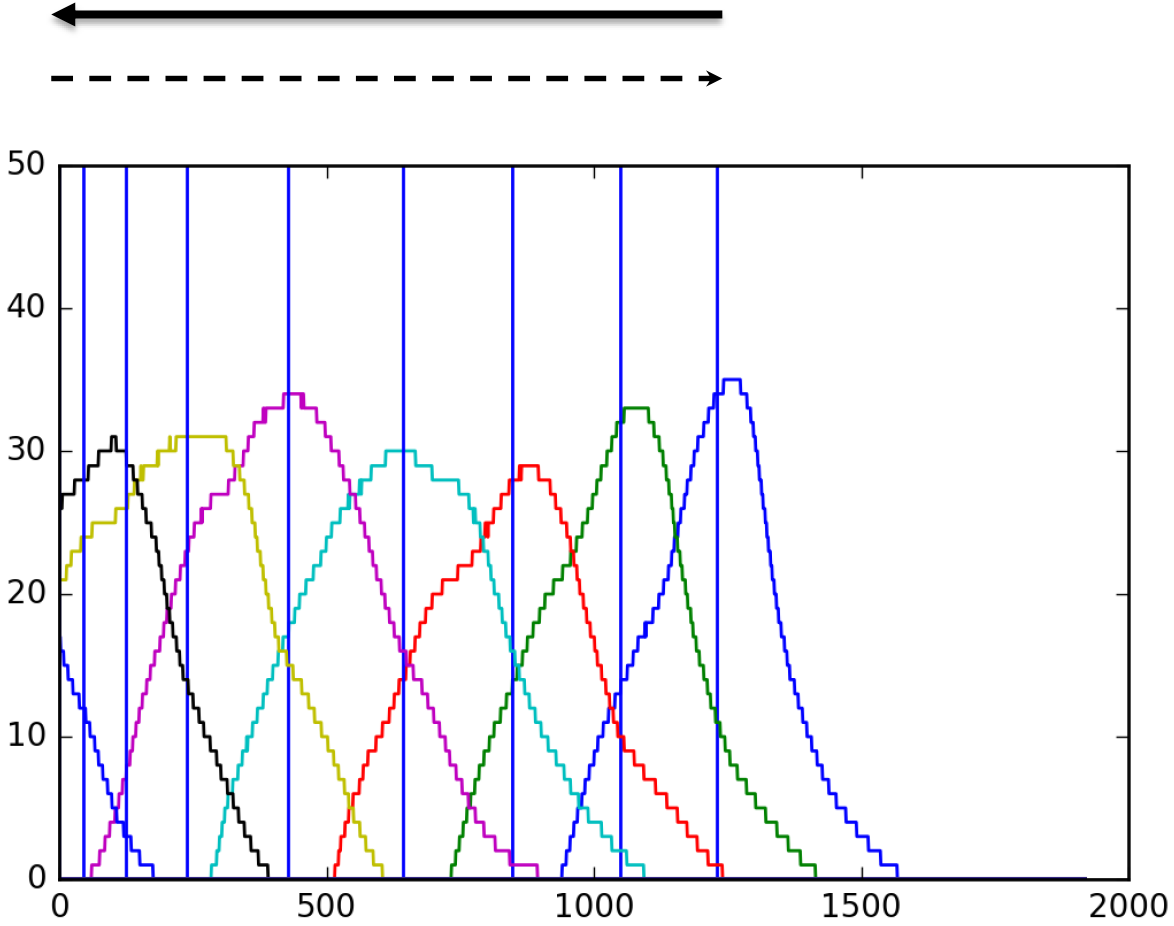
\includegraphics[angle=0,width=14cm]{handcontrol/Bilder/histogramm_schwerpunkt.png}
\caption{Histogramme der Differenzbilder mit Schwerpunkt}
\end{figure}

\section{Entwicklung des Algorithmus}
Der Algorithmus wurde als erstes in MATLAB mit aufgenommenen Videos entwickelt. Nachher wurde auf Python mit OpenCV Binding umgestellt, um einen besseren Vergleich mit der C++ Version zu gewährleisten. Als IDE für Python wurde \href{https://github.com/spyder-ide/spyder}{Spyder} mit dem \href{https://www.continuum.io/downloads}{Anaconda Framework} verwendet. Um den Algorithmus separat von der App zu entwickeln wurde ein "`test\_handcontrol.pro"' Projekt erstellt, welches als eine Art Modultest fungiert. Zu finden in dem schon am Anfang des Kapitels genannten Verzeichnis in Github.

\section{Verbesserungen}
Die Verbesserungen zum Auslesen der Kamera wurden schon in einem separaten Abschnitt behandelt. Für den Algorithmus könnte man statt Grauwertbilder auch Bilder aus dem HSV Raum verwenden. Dort könnte man ggf. Helligkeitsveränderung besser abfangen. Außerdem kann es manchmal vorkommen, dass mehrfach Erkennung erfolgen, diese könnten durch einen Timer abgefangen werden. Eine Verschiebung der Berechnung zur Grafikkarte mittels OpenGL oder OpenCL, wie vorher schon erwähnt, könnte die CPU entlasten und ganz andere Möglichkeiten der Analyse des Frames bieten. Bei der Differenzbildung der Frames entstehen positive und negative Abweichungen, diese könnten in einem verbesserten Algo. separat berücksichtigt werden.


\subsection[Navigation Beschleunigungssensor]{Navigation Beschleunigungssensor\footnote{Jens Helge Micke}}
\thispagestyle{fancy}
\label{Beschleunigungssensor}
\section{Features}
- Blättern in einer Pdf ohne dass ein Update auf dem Server erfolgt\\
\\INOF ans TEAM:Diese Section ist noch nicht fertig
\section{Erweiterungspotential}
Einige zusätzliche Funktionalitäten könnten, den Wert der Applikation für Zuhörer und Sprecher steigern.\\
\\INOF ans TEAM:Diese Section lade ich später hoch
\\INOF ans TEAM:Wenn Ihr die Zuverlässigkeit der Gestensteuerung, Kippsteuerung, Audiosteuerung oder die Sicherheit der Kommunikation noch verbessern wollt, könnt ihr ja wie Tim es in euren Abschnitt einfügen. Hier geht es nur um Erweiterungen der allgemeinen mögliche Funktionalität der Clientapp wie Puplikumsfragen oder sowas.
Erweiterungen für den Sprecher:\\

Erweiterungen für den Zuhörer:\\
- Einstellen der Zeit die vergehen soll bis sich die Applikation synchronisiert\\

-Wartesymbol/Beschäftigungsanzeige
-Touchstgesten
-Audioeinstellungen
-Bildeinstellungen/Wahl der Kamera




\newpage
So kann Code eingefügt werden.
\begin{lstlisting}[frame=single,breaklines=true,basicstyle=\tiny,language=C,label={PWMStart},caption={Kommentierter Start der PWM}]
/*! \brief Starts the PWM
* 
* To make sure that the PWM behaves correctly after a Compare Bit Change the PWM is started and reset with a software trigger.
*/
static void vStartPwm( void )
{
tc_start( &AVR32_TC0, PWM_CHANNEL );
tc_software_trigger( &AVR32_TC0, PWM_CHANNEL );
}
\end{lstlisting}